\documentclass{article}
\usepackage{tikz}
\usepackage{fancyhdr}
\usepackage{geometry}
\usepackage[utf8]{inputenc}
\usepackage[hypertexnames=false, colorlinks=true, linkcolor=black]{hyperref}
\usepackage{listings}
\usepackage{xcolor}
\usepackage{tocloft}
\usepackage{palatino}  % Police
\usepackage{amsmath}
\usepackage{amssymb}
\usepackage{colortbl}
\usepackage{array}
\usepackage[
backend=biber,
style=alphabetic,
]{biblatex}

\usetikzlibrary{backgrounds, shapes.geometric, positioning}

\geometry{a4paper, left=15mm, right=15mm, top=30mm, bottom=30mm}

\pagestyle{fancy}
\fancyhf{}
\fancyhead[L]{Distance de Jaccard}
\fancyhead[R]{Projet Algorithmie 3}
\fancyhead[C]{De-backer Cuvelier Sébastien Llobregat Nicolas}
\fancyfoot[C]{\thepage}

\renewcommand{\contentsname}{Table des matières}

\setlength{\cftbeforesecskip}{20pt}
\setlength{\cftbeforesubsecskip}{10pt}
\setlength{\cftbeforesubsubsecskip}{5pt}

\newcommand{\fondpremierepage}{
  \begin{tikzpicture}[remember picture, overlay]
    \node[align=center, text width=0.8\textwidth, font=\huge\bfseries] at (current page.center) {
        Projet Algorithmie 3 La distance de Jaccard};
    \node[align=center, text width=0.8\textwidth, font=\large] at (current page.center) [yshift=-1.5cm] {
        De-backer Cuvelier Sébastien Llobregat Nicolas};
    \node[align=center, text width=0.8\textwidth, font=\normalsize] at (current page.center) [yshift=-2.5cm] {
        Version du 24 Avril 2025};
  \end{tikzpicture}
}

\lstdefinestyle{Cstyle}{
  language=C,
  basicstyle=\ttfamily\normalsize,       % Style de police (monospace) et taille
  numbers=left,                     % Affichage des numéros de ligne à gauche
  numberstyle=\tiny\color{black},     % Style des numéros de ligne
  stepnumber=1,                     % Numéroter chaque ligne
  numbersep=10pt,                    % Distance entre les numéros et le code
  backgroundcolor=\color{gray!20},     % Fond blanc pour le code
  showspaces=false,                  % Ne pas afficher les espaces
  showstringspaces=true,            % Ne pas afficher les espaces dans les chaînes
  showtabs=false,                    % Ne pas afficher les tabulations
  frame=single,                      % Encadrer le code
  rulecolor=\color{black},           % Couleur de la bordure
  tabsize=2,                         % Taille des tabulations
  captionpos=b,                      % Position de la légende (en bas)
  breaklines=true,                   % Sauter les lignes trop longues
  breakatwhitespace=true,            % Casser à l'espace pour les lignes longues
  morekeywords={long, int, double, return, if, else, while, for, void, switch},  % Ajouter des mots-clés à la coloration
  keywordstyle=\color{brown}\bfseries,  % Colorier les mots-clés en marron et en gras
  commentstyle=\color{gray},         % Colorier les commentaires en gris
  stringstyle=\color{purple}            % Colorier les chaînes en violet
}

\linespread{1.5}

\begin{document}

\fondpremierepage{}
\thispagestyle{empty}

\newpage{}

\tableofcontents

\section{Organisation du travail}

\subsection{Outils utilisés}

\paragraph{Git \& Github :}
Pour la gestion du projet et des différentes versions de celui-ci nous avons fait le choix
d'utiliser un logiciel de versionnage : \textbf{GIT}. Ainsi nous avons pu travailler en 
simultané sur les différentes composantes du projet. La méthodologie était la suivante :
Créations des tâches via les "issues" de \textbf{Github}. Puis création d'une branche spécifique
pour chaque tâche à réaliser. Une fois le travail réaliser nous ouvrons une \textbf{pull request}
pour que notre binôme puisse analyser le travail de l'autre avant de mutualiser sur la branche
principale.

\paragraph{Tests unitaires :}
Nous avions pour ambition d'utiliser les tests unitaires pour s'assurer que chaque fonction
réalisait bien ce qu'elle devait, pour se faire nous avions commencer à utiliser une bibliothèque
qui permettait assez simplement de les réalilser: \textbf{greatest}. Cependant, il s'est avéré
très chronophage et nous avons pris du retard sur ces tests ce qui leur a fait perdre toute utilité.
Nous avons donc choisi de ne pas les inclure dans notre rendu final du projet. 

\subsection{Répartition du travail}

\paragraph{Mesure de la charge de travail :}
Au début du projet, nous n'avions pas réellement conscience de la charge de travail à effectuer.
Il aurait peut-être été intéressant de lors de la première séance de réaliser un planning
avec un tableau de répartition des tâches pour définir une charge de travail équitable. Cependant,
le projet n'étant pas de grande envergure et étant en effectif réduis à deux personnes nous 
avons pu communiquer efficacement pour communiquer sur les tâches que nous étions réalisions. 

\section{Structure du projet}

\paragraph{Origine :}
Lors de la conception de notre binôme nous avons décidé de faire une lecture commune du sujet
afin de savoir si nous avions la même vision. Ainsi nous avons organisé la structure du projet
à l'origine puis nous nous sommes mis d'accord sur les modules à utiliser. Entre les deux
implémentations suggérées soit l'utilisation de \textbf{tables de hachages} ou bien \textbf{d'arbres binaires
de recherches équilibrés}, c'est la deuxième qui nous a convaincu. En effet, il est plus
facile de représenter les arbres et nous avions beaucoup plus travaillé sur cette notion en cours.

\subsection{Les modules}
Les modules utilisés sont: \textbf{avl}, \textbf{jdis}.

\paragraph{Le module jdis :}
Nous avons décidé de créer un module spécifique pour gérer la liaison entre le module \textbf{avl}
et notre utilisation, il consiste principalement à convertir un fichier ou l'entrée standard (voir \textbf{\ref{subsec:stdin}})
en un \textbf{avl}. En le calcul du cardinal de l'intersection des ensembles de mots stockés dans les
arbres. Et bien évidemment au calcul de la distance de Jaccard entre chaque couple deux à deux distincts
des ensembles représentés par les arbres sur laquelle nous reviendrons dans là sous section \textbf{\ref{subsec:jdis}}.

\subsection{Gestion des options}
\paragraph{Généralités :}
Pour ce qui est de la gestion des options, nous avons décidé d'implanter à la fois les options longues et les options courtes.
Les paragraphes qui suivent préciseront ce que ces options font et comment elles le font.

\paragraph{L'option -? / --help :}
Cette option est très simple, elle permet d'afficher le menu d'aide pour l'utilisation 
de notre exécutable et affiche par conséquent des précisions sur les options supportées.

\paragraph{L' option -g / --graph :}
Cette option permet d'afficher un graphe d'appartenance des mots dans les différents 
fichiers passés sur la ligne de commande. Cette fonction est divisée en deux parties.

\begin{lstlisting}[style=Cstyle]
  static int scptr_display(context *ctx, const char *ref); 
\end{lstlisting}
Cette fonction permet d'afficher une ligne du graph, pour se faire le processus est assez simple,
nous allons itérer sur les arbres présents dans le tableau contenu lui-même dans le contexte qui est pris en paramètre.
Ainsi nous allons rechercher la présence de chaque mot présent dans l'arbre de l'union des fichiers dans les arbres, 
le cas échéant nous affichons sur la colonne 'x' indiquant que le fichier contient la référence sinon '-'.
Cette fonction est alors utilisée dans la fonction principale et non statique :
\begin{lstlisting}[style=Cstyle]
  int graph_belonging(bst **t, bst *uni, int nb_file); 
\end{lstlisting}
Celle-ci va utiliser la fonction \textbf{bst\_dft\_infix\_apply\_context} du module \textbf{avl} pour appliquer le traitement
à chauque mot de l'arbre des unions.

\paragraph{L'option -iVALUE / --initial=VALUE :}
Cette option permet de fixer la taille des mots à \textbf{VALUE}.
Celle-ci est traitée au moment de la lecture des mots et permet de signaler qu'il faut ignorer tous les caractères dépassant cette
limite jusqu'au prochain caractère de séparation (voir \textbf{\ref{subsec:fscanf}}). À savoir que par défaut il n'y a pas de limite en
tant que telle, la taille maximale d'un mot sera alors ULONG\_MAX ce qui est plus que raisonnable.

\paragraph{L'option -p / --punctuation-like-space :}
Cette option permet d'indiquer à la fonction de lecture que les caractères de ponctuation de la classe \texttt{isspace} et \texttt{ispunct}
doivent être considérés comme des séparateurs pour segmentation des mots.

\paragraph{L'option \texttt{--} :}
Cette option permet d'échapper l'argument qui suit sur la ligne de commande. Si nous avons un fichier appelé 
\texttt{--help}, par exemple, cette option nous permet de traiter ce fichier comme un fichier et non comme l'option \textbf{--help} ci-dessus.
Cela se fait tout simplement par le fait d'effectuer le test de comparaison de la présence de l'option en premier afin de stocke rle nom du fichier.

\paragraph{L'option \texttt{-} :}
Cette dernière option permet de rentrer des mots sur l'entrée standard pour qu'ils soient traité comme un fichier (voir \textbf{\ref{subsec:stdin}}).

\subsection{Gestions des fichiers}\label{subsec:files}
Pour gérer les fichiers pris en arguments par le programme nous ouvrons simplement le fichier
associé en mode lecture seule puis nous lisons (précisions \textbf{\ref{subsec:fscanf}}) chaque
mot et nous tentons de l'ajouter à l'arbre binaire associé. À la fin de la lecture, nous avons
un arbre contenant des pointeurs vers les mots. Il est à noté que pour un même fichier, on stocke
en un et un seul exemplaire les mots apparaissant plusieurs fois dans le même fichier. Nous avons un
tableau avec l'ensemble des arbres créer.

\paragraph{Exemple :}
Ainsi si nous exécutons la commande suivante : \colorbox{lightgray!20}{\textit{./jdis x0.txt x1.txt x2.txt}}
où les fichiers x0.txt et x1.txt sont ceux donnés dans le sujet du projet, nous aurons la représentation
suivante :
\begin{center}
  \begin{tikzpicture}
    \node (case1) at (0, 0) [rectangle, draw, minimum width=1cm, minimum height=3cm] {x2.txt};
    \node (case2) at (0, -3) [rectangle, draw, minimum width=1cm, minimum height=3cm] {x1.txt};
    \node (case3) at (0, -6) [rectangle, draw, minimum width=1cm, minimum height=3cm] {x0.txt};
    
    \node at (-1, 0) {\textbf{\textcolor{red}{2}}};
    \node at (-1, -3) {\textbf{\textcolor{red}{1}}};
    \node at (-1, -6) {\textbf{\textcolor{red}{0}}};
    \node at (0, 2) {\textbf{\textcolor{red}{t}}};

    \draw[->, bend right=25] (case1) to node[below] {} (-5.78, 2.5);
    \draw[->, bend right=25] (case2) to node[below] {} (-5.7, -3.5);
    \draw[-] (case3) to node[below] {} (2, -3.5);
    \draw[->, bend left=40] (2, -3.5) to (3.85, -3);
      
      \node at (-6, 0.25) {
        \begin{tikzpicture}[
          scale=0.60,
          sibling distance=70mm,
          level distance=20mm,
          every node/.style={draw, fill=gray!20, circle},
          edge from parent/.style={draw, thick},
          level 1/.style={sibling distance=80mm},
          level 2/.style={sibling distance=40mm},
          level 3/.style={sibling distance=20mm}
        ]
          \node {dddd}
            child { node {bb}
                child { node {a} }
                child { node {ccc} }
            }
            child { node {hhhh}
                child { node {ffffff}
                child { node {eeeee} }
                child { node {ggggg} }
            }
                child { node {jj} 
                child { node {iii} }  
                child { node {k} }  
              }
            };
        \end{tikzpicture}
          
      };
      
      \node at (-6, -4.85) {
          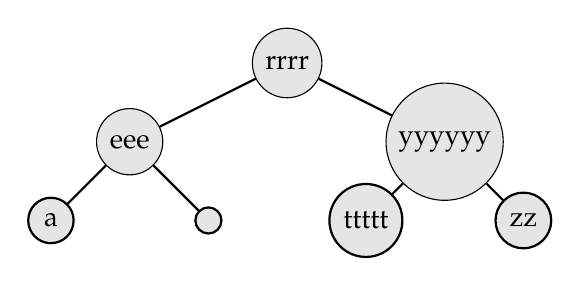
\begin{tikzpicture}[
            scale=0.5,
            sibling distance=70mm,
            level distance=20mm,
            every node/.style={draw, fill=gray!20, circle},
            edge from parent/.style={draw, thick},
            level 1/.style={sibling distance=80mm},
            level 2/.style={sibling distance=40mm},
            level 3/.style={sibling distance=20mm}
          ]
            \node {rrrr}
              child { node {eee}
                  child { node {a} }
                  child { node {} }
              }
              child { node {yyyyyy}
                  child { node {ttttt} }
                  child { node {zz} }
              };
          \end{tikzpicture}
      };
      
      \node at (4.5, -4.5){
        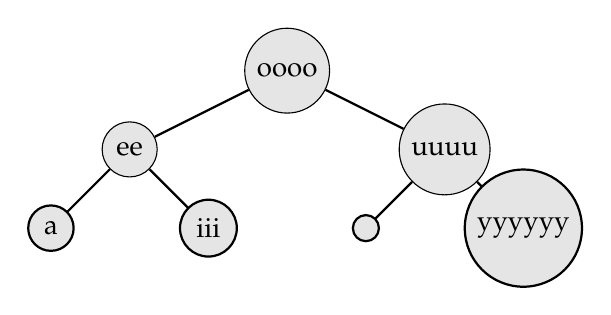
\begin{tikzpicture}[
          scale=0.5,
          sibling distance=70mm,
          level distance=20mm,
          every node/.style={draw, fill=gray!20, circle},
          edge from parent/.style={draw, thick},
          level 1/.style={sibling distance=80mm},
          level 2/.style={sibling distance=40mm},
          level 3/.style={sibling distance=20mm}
        ]
          \node {oooo}
            child { node {ee}
                child { node {a} }
                child { node {iii} }
            }
            child { node {uuuu}
                child { node {} }
                child { node {yyyyyy} }
            };
        \end{tikzpicture}
      };
  \end{tikzpicture}
\end{center}

\begin{center}
  \colorbox{lightgray!20}{\textit{\underline{Exemple 1: Conversion d'un fichier en arbre}}}
\end{center}

\subsection{Gestion de l'entrée standard}\label{subsec:stdin}
\paragraph{Questionnement :}
Nous avons réfléchi comment traiter l'argument particulier \textbf{'-'}, deux Choix
s'offraient alors à nous, créer l'arbre depuis l'entrée standard directement ou bien de stocker l'entrée standard dans un fichier
puis effectuer le même traitement que sur les autres arguments sans distinction aucune. Par soucis d'efficacité,
c'est donc la première solution qui a été choisie. Dans le cas où l'on détecte '-' à la place d'un nom de fichier alors nous avons plus
qu'à lire depuis l'entrée standard.

\section{Choix d'implémentation}

\subsection{Stockage des mots avec holdall}
\paragraph{Généralités :}
Dans un premier temps nous avons eu recourt au module \textbf{holdall} pour le stockage des mots, 
afin de séparer le traitement des mots de la gestion en mémoire. Nous aurions pu choisir d'utiliser la fonction
\textbf{bst\_dft\_infix\_apply\_context} du module \textbf{avl} pour libérer les ressources.
Nous avons également décider de tester cette solution en parallèle et nous en faisons référence dans
la section \textbf{\ref{sec:perf}} liée aux performances de l'implémentation proposée.
Deux versions de ce module ont été réfléchis pendant la création de ce projet. La première en utilisant le 
principe des listes dynamiques simplement chainées et la seconde en utilisant les tableaux dynamiques.
\subsubsection{Implémentation par LDSC}\label{subsec:impl}
Pendant les cours d'algorithmique, nous avons étudié les listes dynamiques simplement chaînées (LDSC).
Ce type de structure permet d'ajouter rapidement des éléments en tête de liste, en temps constant,
ce qui est très avantageux en termes de performance. En effet, chaque ajout nécessite juste de créer
un nouveau maillon et de modifier un pointeur, sans avoir à déplacer d'autres éléments. 
Cependant, cette rapidité a un coût : chaque maillon prend plus de mémoire, car il contient un pointeur en 
plus de la donnée. Cela devient encombrant quand les fichiers sont volumineux. De plus, l'accès à un élément précis 
est plus lent, car il faut parcourir la liste depuis le début.
\subsubsection{Implémentation par tableaux dynamiques}
Pour résoudre le problème d'espace, nous avons pensé aux tableaux dynamiques. En effet l'avantage, ici,
est que les ajouts se font également en temps constant grâce à un accès direct aux cellules du tableau et nous n'avions
pas besoin d'allouer toute une cellule de liste pour un seul mot ; nous avions juste à allouer un tableau assez grand pour
stocker les mots. Pour les petits fichiers cette implémentation s'est montré très efficace, mais pour les gros fichiers
le programme passait énormément de temps à recopier les données déjà présentes dans le tableau.

\paragraph{Conclusion :}
Nous avons finalement décidé de ne pas utiliser ce module pour avoir une performance optimale sur notre exécutable.
Néanmoins, nous avons réalisé une petite étude sur un petit jeu de données afin de se rendre compte des différences.

\section{Calcul de la distance de Jaccard :}\label{subsec:jdis}
\paragraph{Les paires distinctes :}
Nous avons maintenant notre tableau avec des pointeurs vers nos arbres, on peut
rappeler que la taille d'un arbre s'effectue en temps contant dans le contrôleur.
Nous allons avoir à calculer la distance de Jaccard entre chaque couple deux à deux
distincts d'arbres. Pour cela il suffit d'avoir deux boucles imbriquées : 
\newpage{}
\begin{lstlisting}[style=Cstyle]
for (int i = 0; i < k - 1; ++i) {
  for (int j = i + 1; j < k; ++j) {
    . . .
  }
}  
\end{lstlisting}
\underline{La première boucle :} nous commençons à $i = 0$ et allons jusqu'à $i = k - 2$ (car $i < k - 1$)\\
\underline{La deuxième boucle :} pour chaque valeur de $i$ nous commençons à $j = i + 1$ et va 
jusqu'à $j = k - 1$ (car $j < k$).
L'idée ici est de parcourir chaque combinaison unique de $i$ et $j$ où $i$ est strictement inférieur à $j$. 
Cela permet de créer une paire unique sans répéter les mêmes éléments dans les deux positions.

\paragraph{Rappel sur la distance de Jaccard:}
Nous devons maintenant effectuer le calcul de la distance de jaccard, petit rappel sur la formule :
La \textbf{distance de Jaccard} entre deux ensembles \( A \) et \( B \) est définie par la formule suivante :

\[
J_{\delta}(A, B) = 
\begin{cases} 
0 & \text{si } A = \emptyset \wedge B = \emptyset, \\
1 - \frac{|A \cap B|}{|A \cup B|} & \text{sinon.} \\
\end{cases}
\]

\paragraph{Calcul du cardinal de l'union :}
Nous avons donc besoin du cardinal de l'intersection ainsi que le cardinal de l'union de chaque couple,
pour cela nous allons en réalité ne calculer que le cardinal de l'intersection. En effet, nous allons utiliser
une petite astuce de la théorie des ensembles qui nous dit que : Le cardinal de l'union de deux ensemble ce n'est rien d'autre
que la somme de leurs cardinaux respectifs moins le cardinal de l'intersection. On peut facilement s'en rendre compte ici:

\begin{center}
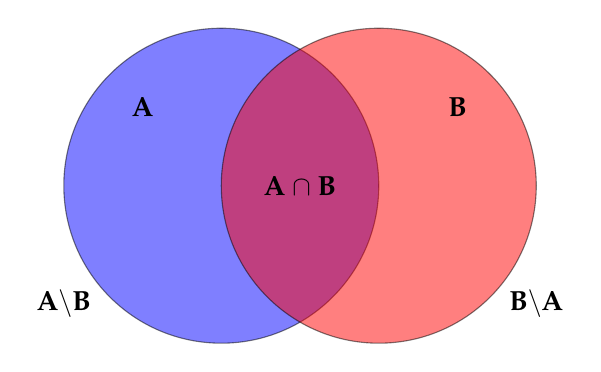
\begin{tikzpicture}
  \draw[fill=blue,opacity=0.5] (0,0) circle(2);
  \draw[fill=red,opacity=0.5] (2,0) circle(2);

  \node at (-1,1) {\textbf{A}};
  \node at (3,1) {\textbf{B}};

  \node at (1,0) {\textbf{A $\cap$ B}};
  \node at (-2,-1.5) {\textbf{A$ \setminus $B}};
  \node at (4,-1.5) {\textbf{B$ \setminus $A}};  
\end{tikzpicture}
\end{center}
\begin{center}
  \colorbox{lightgray!20}{\textit{\underline{Schéma 1: Généralités sur les ensembles}}}
\end{center}

\paragraph{Calcul du cardinal de l'intersection}
Nous devons alors calculer l'intersection des deux ensembles, pour cela nous allons de nouveau
utiliser la fonction \textbf{bst\_dft\_infix\_apply\_context} du module \textbf{avl}. Cette fois-ci 
nous allons un contexte qui sera une structure contenant un compteur ainsi que le plus petit des deux 
ensembles. Ansi, nous allons parcourir le plus grand des deux et rechercher dans le plus petit la référence 
grâce à la fonction \textbf{bst\_search} du module \textbf{avl}. Si on la trouve alors on ajoute un au compteur
cela veut dire qu'elle se trouve dans les deux sinon non. À la fin dans le contexte, nous aurons le cardinal de l'ensemble.

\paragraph{Calcul final :}
Il nous reste plus qu'à rassembler les éléments, ainsi nous avons :
Un moins le cardinal de l'intersection divisé par la taille des deux arbres moins le cardinal de l'intersection ce qui nous donne
la distance de Jaccard entre les deux ensembles de mots de la paire de fichiers. On peut alors réitéré sur toutes les paires.

\section{Les difficultés rencontrées}

\subsection{Tentative d'utilisation de getopt}
\paragraph{La bibliothèque getopt :} 
En premier lieu nous nous sommes intéressés à la bibliothèque getopt qui nous permettait de parser 
la ligne de commande pour trouver les options notamment grâce à \textbf{optind} et \textbf{optarg}. Nous pouvions également préciser 
quelles options nécessitaient des paramètres comme pour l'option qui permet de fixer la taille 
maximale des mots \textbf{-iVALUE} ou \textbf{--initial=VALUE}. Grâce à \textbf{getopt}
nous avons pu implanter les options très rapidement, mais nous avons rencontré un problème 
lorsque nous voulions implanter l'option '--' permettant d'échapper le nom d'un fichier.
En effet, lorsque nous utilisions cette option, nous avons remarqué quelle échappait tous les 
paramètres qui suivaient. Nous avons d'abord cherché une solution en remplaçant \textbf{getopt}
par \textbf{getopt\_long}. Ce qui nous compliquait la tâche. Finalement il a été choisi de parser
nous même la ligne de commande pour avoir un contrôle total sur son traitement.

\subsection{La fonction fscanf}\label{subsec:fscanf}
\paragraph{utilisation de fscanf :}
Afin de créer les arbres comme nous l'avons décrit dans la section \textbf{\ref{subsec:files}} nous avons
besoin de lire dans les fichiers, pour se faire il convient d'usage d'utiliser la fonction \textbf{fscanf}, et c'est le choix
que nous avions fait lors de la première partie du projet cependant, après avoir essayé d'implémenter l'option 
-p (resp. --punctuation-like-space) nous avions un problème de compréhension de la fonction. Il fallait de plus
analyser une deuxième fois le buffer que nous prenions afin de l'analyser par la suite. En outre cela revenait à lire chacun des caractères
deux fois et donc de doubler la compléxité temporelle. Il a été alors naturellement convenu de coder notre propre
fonction de lecture  d'où l'apparition de la fonction statique \textbf{hm\_\_fscanf} (hm pour home maid). Ainsi nous lisons
caractère par caractère dans le fichier donné par la tête de lecture en paramètre grâce à la fonction \textbf{fgetc}.
Elle permet de gèrer en une seule fois le cas où nous devons prendre en compte la ponctuation ou non.

\section{Performances}\label{sec:perf}
\paragraph{Analyse de quelques données :}
Nous allons analyser quelques données afin d'avoir une idée de la performance de notre executable, nous verrons ensuite
une étude théorique afin de conformer nos observations, enfin nous donnerons quelques pistes d'améliorations.\\\\
\textbf{Avec le module holdall implémenté par LDSC:}
\begin{center}
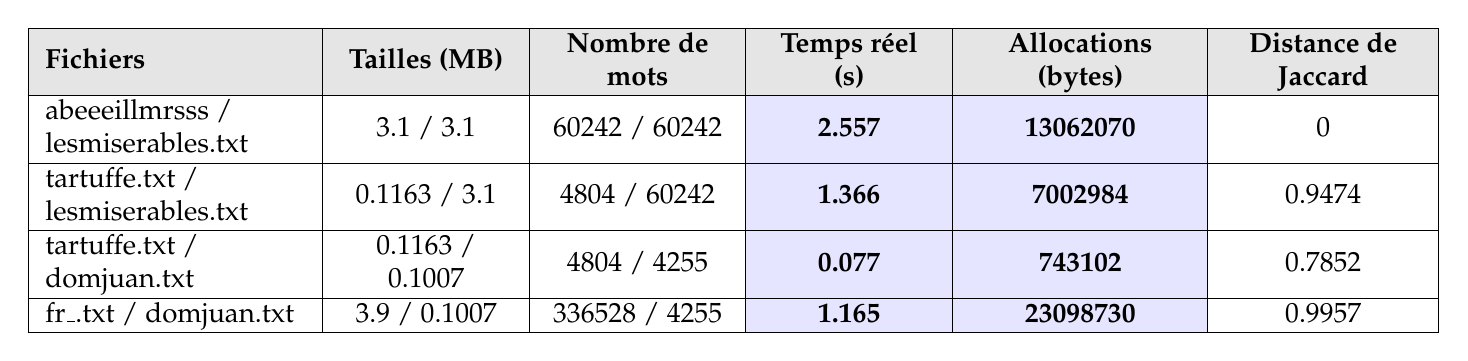
\begin{tikzpicture}
  \node[inner sep=0pt] (table) {
    \begin{tabular}{|>{\raggedright\arraybackslash}m{3.3cm}|
      >{\centering\arraybackslash}m{2.2cm}|
      >{\centering\arraybackslash}m{2.3cm}|
      >{\columncolor{blue!10}\centering\arraybackslash}m{2.2cm}|
      >{\columncolor{blue!10}\centering\arraybackslash}m{2.8cm}|
      >{\centering\arraybackslash}m{2.5cm}|}  
      \hline
  \rowcolor{gray!20}
  \textbf{Fichiers} & \textbf{Tailles (MB)} & \textbf{Nombre de mots} & \textbf{Temps réel (s)} & \textbf{Allocations (bytes)} & \textbf{Distance de Jaccard} \\
  \hline
  abeeeillmrsss / lesmiserables.txt & 3.1 / 3.1 & 60242 / 60242 & \textbf{2.557} & \textbf{13062070} & 0 \\
  \hline
  tartuffe.txt / lesmiserables.txt & 0.1163 / 3.1 & 4804 / 60242 & \textbf{1.366} & \textbf{7002984} & 0.9474 \\
  \hline
  tartuffe.txt / domjuan.txt & 0.1163 / 0.1007 & 4804 / 4255 & \textbf{0.077} & \textbf{743102} & 0.7852 \\
  \hline
  fr\_.txt / domjuan.txt & 3.9 / 0.1007 & 336528 / 4255 & \textbf{1.165} & \textbf{23098730} & 0.9957 \\
  \hline
  \end{tabular}
  };
\end{tikzpicture}
\end{center}
\textbf{Avec le module holdall implémenté par tableaux dynamiques avec gestion préfixielle:}
\begin{center}
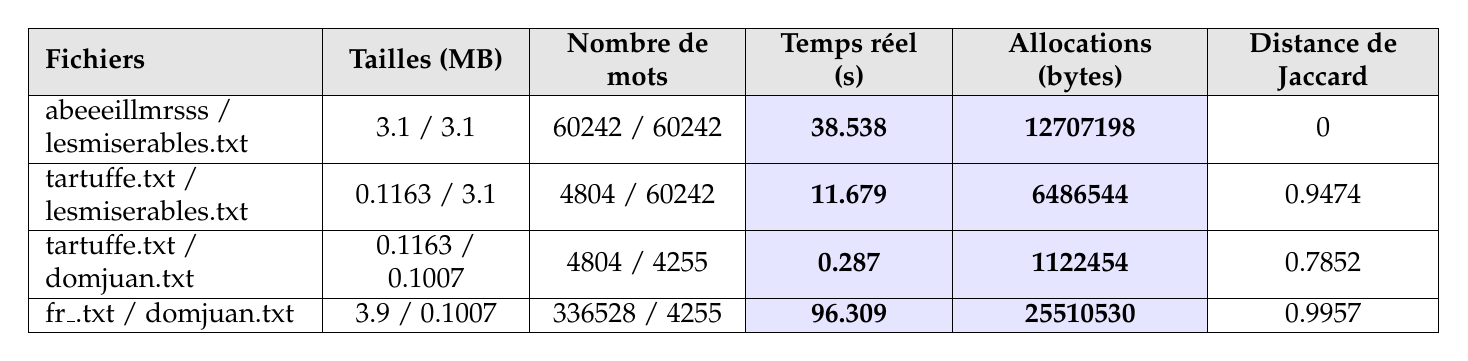
\begin{tikzpicture}
  \node[inner sep=0pt] (table) {
    \begin{tabular}{|>{\raggedright\arraybackslash}m{3.3cm}|
      >{\centering\arraybackslash}m{2.2cm}|
      >{\centering\arraybackslash}m{2.3cm}|
      >{\columncolor{blue!10}\centering\arraybackslash}m{2.2cm}|
      >{\columncolor{blue!10}\centering\arraybackslash}m{2.8cm}|
      >{\centering\arraybackslash}m{2.5cm}|}  
  \hline
  \rowcolor{gray!20}
  \textbf{Fichiers} & \textbf{Tailles (MB)} & \textbf{Nombre de mots} & \textbf{Temps réel (s)} & \textbf{Allocations (bytes)} & \textbf{Distance de Jaccard} \\
  \hline
  abeeeillmrsss / lesmiserables.txt & 3.1 / 3.1 & 60242 / 60242 & \textbf{38.538} & \textbf{12707198} & 0 \\
  \hline
  tartuffe.txt / lesmiserables.txt & 0.1163 / 3.1 & 4804 / 60242 & \textbf{11.679} & \textbf{6486544} & 0.9474 \\
  \hline
  tartuffe.txt / domjuan.txt & 0.1163 / 0.1007 & 4804 / 4255 & \textbf{0.287} & \textbf{1122454} & 0.7852 \\
  \hline
  fr\_.txt / domjuan.txt & 3.9 / 0.1007 & 336528 / 4255 & \textbf{96.309} & \textbf{25510530} & 0.9957 \\
  \hline
  \end{tabular}
  };
\end{tikzpicture}
\end{center}
\textbf{Sans le module holdall en libérant les ressources avec la fonction bst\_dft\_infix\_apply\_context du module avl :}

\begin{center}
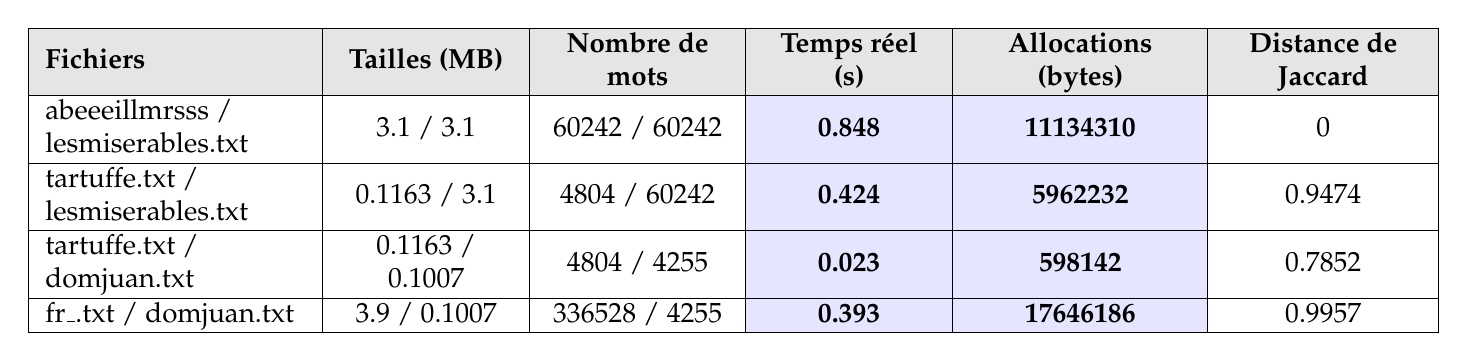
\begin{tikzpicture}
  \node[inner sep=0pt] (table) {
  \begin{tabular}{|>{\raggedright\arraybackslash}m{3.3cm}|
                  >{\centering\arraybackslash}m{2.2cm}|
                  >{\centering\arraybackslash}m{2.3cm}|
                  >{\columncolor{blue!10}\centering\arraybackslash}m{2.2cm}|
                  >{\columncolor{blue!10}\centering\arraybackslash}m{2.8cm}|
                  >{\centering\arraybackslash}m{2.5cm}|}
  \hline
  \rowcolor{gray!20}
  \textbf{Fichiers} & \textbf{Tailles (MB)} & \textbf{Nombre de mots} & \textbf{Temps réel (s)} & \textbf{Allocations (bytes)} & \textbf{Distance de Jaccard} \\
  \hline
  abeeeillmrsss / lesmiserables.txt & 3.1 / 3.1 & 60242 / 60242 & \textbf{0.848} & \textbf{11134310} & 0 \\
  \hline
  tartuffe.txt / lesmiserables.txt & 0.1163 / 3.1 & 4804 / 60242 & \textbf{0.424} & \textbf{5962232} & 0.9474 \\
  \hline
  tartuffe.txt / domjuan.txt & 0.1163 / 0.1007 & 4804 / 4255 & \textbf{0.023} & \textbf{598142} & 0.7852 \\
  \hline
  fr\_.txt / domjuan.txt & 3.9 / 0.1007 & 336528 / 4255 & \textbf{0.393} & \textbf{17646186} & 0.9957 \\
  \hline
  \end{tabular}
  };
\end{tikzpicture}
\end{center}


\paragraph{Conclusion :}
Il est évident que la version sans holdall est bien plus performante. 

\newpage{}
\paragraph{\textbf{Précisions sur les résultats obtenus:}}

\paragraph{Avec LDSC :} Comme nous pouvons le remarquer dans le premier tableau, les statistiques temporelles sont relativement satisfaisantes 
lorsque nous les comparons avec celles relevant d'une implémentation par tableaux dynamiques. Ce qui pose problème ici, c'est le nombre d'allocations.
En effet, ce nombre est le plus élevé des trois implémentations ci-dessus. Ce qui est cohérent puisque nous allouons une cellule de liste qui contient
\texttt{la référence} et un champ \texttt{next} pour chaque mot trouvé dans les fichiers.
Nous pouvons donc l'améliorer en essayant de réduire le nombre d'allocations.

\paragraph{Par tableaux dynamiques :} Ce qui, à première vue, semblait une amélioration possible de notre projet, c'est avérée la pire implémentation de
celles proposées dans notre projet. Nous avions effectivement réduit le nombre d'allocations par rapport au LDSC, mais nous perdions un temps considérable
à recopier le tableau dynamique lorsque celui-ci était trop petit. Comme nous pouvons le voir nous avons environ 39 secondes pour traiter les fichiers\\
\textbf{\texttt{abeeeillmrsss.txt}} et \textbf{\texttt{lesmiserables.txt}}. Nous ne pouvions pas rester sur cette implémentation.

\paragraph{Sans module \texttt{Holdall:}} En effet supprimer totalement ce module permettrais de supprimer beaucoup d'allocations et donc de gagner du temps.
De plus nous stockons déjà toutes les références des mots dans les "AVL fichiers", nous avons donc utilisé la fonction \textbf{bst\_dft\_infix\_apply\_context}
pour nous permettre de parcourir tous les AVL et ainsi libérer les références. Et cette méthode, c'est avérée la meilleure au vu des résultats. Avec les mêmes 
textes cités précédemment nous avons pu diviser le temps par 45 par rapport à l'implémentation par tableau dynamique, et environ 2M d'octets de gagnés 
par rapport au LDSC.

\section{Améliorations possibles}

\paragraph{Une implémentation totalement différente :} Nous avons remarqué grâce à l'exécutable fourni sur universitice 
que nous pouvions faire bien mieux en utilisant les tables de hachages. En effet, en utilisant une table de hachage qui contiendrait
tous les mots distincts en tant que clés et l'appartenance dans les fichiers en tant que valeurs, nous aurions eu besoin d'allouer 
seulement la table de hachage ; là où, pour notre projet, nous avions besoin d'un AVL par fichiers et également un AVL d'union totale 
pour l'affichage du graphe lorsque celui-ci est demandé. Nous perdons donc beaucoup de temps à allouer les ressources nécessaires. 

\paragraph{N'allouer qu'une seule fois les références :} Un autre problème de notre implémentation, c'est vu qu'on créér un AVL par fichier
ce qui cause plusieurs allocations d'un même mot lorsque celui-ci existe dans plusieurs fichiers. La solution serait de stocker des pointeurs
vers les références, qui elles sont uniques, dans les AVL. Nous avions déjà pensé à cette solution avant mais ne pouvions pas le coder vu 
les restrictions données dans le sujet, c'est-à-dire : 
\begin{center}
  \textbf{"vous utiliserez nécessairement soit l’en-tête \texttt{hashtable.h}, soit
  l’en-tête \texttt{bst.h}, \underline{sans les modifier}"}
\end{center}

\end{document}
